\chapter{Sound Event Localization and Detection}
\label{chap:seld2019}


%%%%%%%%%%%%%%%%%%%%%%%%%%%%%%%%%%%%%%%%%%%%%%%%%%%%%%%%%%%%
%%%%%%%%%%%%%%%%%%%%%%%%%%%%%%%%%%%%%%%%%%%%%%%%%%%%%%%%%%%%
\section{Introduction}
\label{sec:intro}
%


Sound Event Localization and Detection (SELD) refers to the problem of identifying, for each individual event present in a sound field, the \textbf{spatial location} $\Omega$, \textbf{temporal activity} $\Upsilon$, and \textbf{sound class} $\kappa$ to which it belongs. 

The organization of a dedicated SELD task within the IEEE AASP Challenge on Detection and Classification of Acoustic Scenes and Events (DCASE) 2019 can be considered as a milestone for the development of the SELD research problem. 
Indeed, a large number of novel methodologies were developed for the Challenge, most of them based on Convolutional Recurrent Neural Networks (CRNN). The performance of the baseline method, a CRNN that performed jointly the localization and classification tasks \cite{Adavanne2018_JSTSP}, was vastly exceeded by a variety of deep-learning based algorithms \cite{kapka2019sound, Cao2019, grondin2019sound}.
Some of these improvements have been included in the baseline system for the SELD Challenge of DCASE 2020. 

Despite the predominant trend towards high-complexity deep-learning architectures, some recent works have been able to match or even improve CRNN-based methods with regard to localization, by using parametric analysis of the ambisonic sound field \cite{perez2019hybrid, nguyen2020sequence}.  
Apart from the benefit derived by their simplicity, these approaches are able to resolve the case of overlapping events of the same class, a situation difficult to disambiguate for CRNN-based methods \cite{politis2020dataset}.


The present work continues the exploration of possibilities of parametric SELD methods, focusing on a low-complexity architecture that makes use of traditional, feature-based machine learning techniques. The method has been developed in the context of the SELD task within DCASE 2020 Challenge, and therefore utilizes the proposed dataset, baseline system and evaluation metrics.

Finally, it is important to remark that the method described here is the continuation of an algorithm presented at the DCASE 2019 Challenge \cite{perez2019hybrid}; both algorithms share a common structure and a similar approach to the SELD problem. 
However, the current proposal tries to solve some of the problems identified on our early approach, mainly related with a low frame recall derived from a naive approach to event segmentation. Moreover, the current method also presents a complexity reduction, regarding the single-source 
DOA estimation and the classifier. 


%%%%%%%%%%%%%%%%%%%%%%%%%%%%%%%%%%%%%%%%%%%%%%%%%%%%%%%%%%%%
%%%%%%%%%%%%%%%%%%%%%%%%%%%%%%%%%%%%%%%%%%%%%%%%%%%%%%%%%%%%
\section{SYSTEM DESCRIPTION}
\label{sec:methodology}

The proposed method, referred to as \textit{PAPAFIL}, can be summed up in four steps:

\begin{enumerate}
    \item Estimate single-source time-frequency bins.
    \item Use a particle tracking system to estimate event trajectories and activation times from single-source bins.
    \item Perform spatio-temporal filtering on the input signal.
    \item Assign a class label to the estimated event.
    % \item The estimated event is assigned a class label by a classifier.
\end{enumerate}

A scheme of the method is shown in Fig.~\ref{fig:scheme}.

\begin{figure}[th!]
  \centering
  \centerline{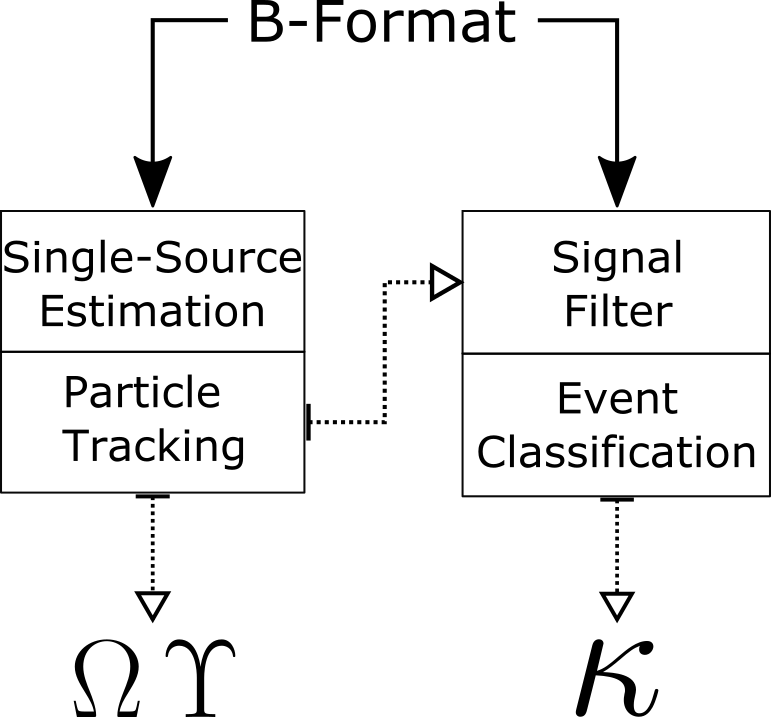
\includegraphics[width=0.75\textwidth]{Figures/SELD/ARCH.png}}
  \caption{Architecture of the proposed methodology.}
  \label{fig:scheme}
\end{figure}


%%%%%%%%%%%%%%%%%%%%%%%%%%%%%%
\subsection{Single-source estimation}

The first step is the transformation of the B-Format input signal $x_n^m(t)$ using the Short-Time Fourier Transform (STFT) into the time-frequency (TF) signal $X_n^m(k,n)$.

In the resulting spectrogram, the frequencies above a given limit $f_{max}$ are discarded; this procedure speeds up the method while maintaining the directional information, given that the microphone geometry aliases spatial measurements above approx. 5 kHz \cite{Bertet2006}.

Assuming that the sources are sparse in time-frequency, it could be possible to identify TF bins which contain a significant energetic contribution from only one source.
% i.e., without significant cross-talk from other sources or background noise. 
These bins could be then used to produce accurate DOA estimates. The effectiveness of this approach has already been demonstrated \cite{tho2014robust, nguyen2020sequence}.

Single-source TF bins are computed from the DirAC parametric analysis.
A variety of alternative subspace methods are known \cite{epain2016spherical, madmoni2018direction}; however, those methods require local estimation of eigenvalues, which is a computationally expensive procedure. 
% This is the main reason for the choice of DirAC-based analysis in this work. 

A TF bin is counted as single-source if its diffuseness $\Psi(k,n)$ is lower than a threshold $\Psi_{max}$. Diffuseness is computed here using Eq.~\ref{eq:psidefinition}. 
 Finally, the DOA $\Omega(k,n)$ of the TF bins passing the aforementioned single-source test is computed as the angle of the active intensity vector by Eq.~\ref{eq:doa}.
 To illustrate the process, an example of the method output is plotted in Fig.~\ref{fig:plots} (top).
% As an example, Fig.~\ref{fig:plots} (top) plots the estimated DOAs of single-source TF bins.

\begin{figure}[th!]
  \centering
  \centerline{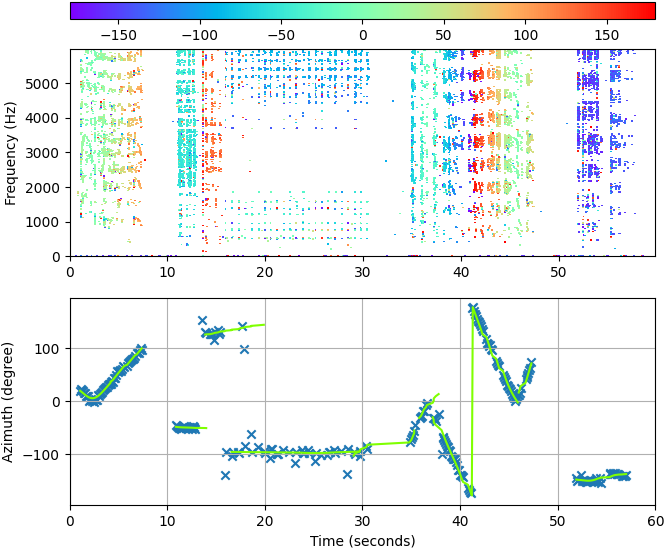
\includegraphics[width=\columnwidth]{Figures/SELD/plots.png}}
  \caption{Estimation of localization and temporal activation. Top: azimuth spectrogram after diffuseness mask; color indicates estimated position of a TF bin passing the single-source test. Bottom: input/output of the particle tracking; the crosses represent the measurement space, and the continuous lines are the resulting events.}
  \label{fig:plots}
\end{figure}

 

%%%%%%%%%%%%%%%%%%%%%%%%%%%%%%
\subsection{Particle tracking}

Once a set of reliable TF DOA estimates is obtained, the next step is the generalization of the individual measurements into trajectories and temporal activations.
% Given that the instantaneous number of sources is unknown, it is necessary to use a multiple target tracker. 
In our case, we opted for the Rao-Blackwellized Monte-Carlo Data Association (RBMCDA) algorithm \cite{sarkka2004rao}, which decomposes the multiple target tracking problem in two: it solves first the data association problem, and then performs the single target tracking individually. 
This method has been recently used in the context of sound event localization and tracking with successful results \cite{Adavanne2018_JSTSP, adavanne2019localization}; the code used for our implementation has been adapted from the same authors\footnote{\url{https://github.com/sharathadavanne/multiple-target-tracking}}.

The system takes as the input the set of TF DOA values passing the single source test, and produces spatio-temporal event trajectories, considering an event as an entity with contiguous temporal activation and continuous spatial position. 
More specifically, for each time frame of the DOA masked spectrogram, the median\footnote{Circular median in the case of azimuth.} of all narrowband DOA estimates is computed. The resulting value is added to the measurement space of the tracker if the number of single-source frequency bins for that frame exceeds a minimum $K_{min}$. 

The performance of the RBMCDA algorithm is controlled by several parameters. Some of the most relevant include the angular velocity prior $v$, the standard deviation $\sigma_{\nu}$ and the spectral density $s_{\nu}$ of the measurement noise, the prior probabilities of birth $p_{birth}$ and noise percentage $p_{\nu}$, and the number of Monte-Carlo particles $N$. Position-related parameters are adjusted with respect to their ranges, so that azimuth-related magnitudes double elevation values.  



The procedure is followed by a numerical post-processing step, which includes data interpolation, resampling (if needed), and removal of elements shorter than $T_{min}$.
Finally, the system provides a list of $J$ events, each one having an instantaneous position $\Omega_j(t)$ and a temporal activation $\Upsilon_j$. 
An example of the system inputs and outputs is depicted in Fig.~\ref{fig:plots} (bottom).



 
%%%%%%%%%%%%%%%%%%%%%%%%%%%%%%
\subsection{Signal filter}

The information provided by the particle tracking system is used to spatially filter the input signal. This can provide an enhanced monophonic estimate of an event $\tilde{s}_j(t)$ with reduced influence of simultaneous events.
The process is performed by steering a virtual first-order cardioid in the direction of interest, using Eq.~\ref{eq:decoding}.
%\begin{equation}
%	\tilde{s}_j(t) = \sum_{m=0}^{M-1} x_m(t) Y_m(\Omega_j) \alpha_n
%	\label{eq:decoding}
%\end{equation}
%where $\bm{Y}(\Omega_j) = [Y_0(\Omega_j), \dots, Y_3(\Omega_j)]^\intercal$ are the real-valued spherical harmonics up to first order evaluated in the direction $\Omega_j$ \cite{daniel2000representation}, and the column vector $\alpha_n$ controls the beam pattern directivity.
 The result of this process is a monophonic estimate for each event, $\tilde{s}_j(t)$, temporally delimited by $\Upsilon_j$. 
 As a last step, each estimate is amplitude peak-normalized, in order to minimize potential amplitude variability due to arbitrary configurations of the scene. 


%%%%%%%%%%%%%%%%%%%%%%%%%%%%%%
\subsection{Event classification}
As a final step, a class label is assigned to each estimated event $\tilde{s}_j(t)$ using a single-class classifier. Since the objective is to keep complexity low and make results interpretable, a machine learning algorithm is used instead of deep learning frameworks. The main advantages of this choice are: (i) low number of parameters; (ii) low train and predict computational time, easing reproducibility; and (iii) relative importance of the features in the output can be interpreted, which is not possible with deep learning approaches.

Gradient Boosting Machine (GBM, Fig.~\ref{fig:gbm}) has been selected as the classification algorithm since it is a powerful yet simple technique for predictive modeling. 
In essence, the algorithm is aimed to minimize the loss of the objective function by adding many weak learners. These learners are typically simple decision trees and their parameters are tuned using gradient descent techniques. 
GBM implementation makes use of the \textit{scikit-learn} library \cite{scikit-learn}.
% Specifically, XGBoost framework is implemented for training process due to its proven performance in a wide range of classification problems \cite{xgboost}.

\begin{figure}[t]
  \centering
  \centerline{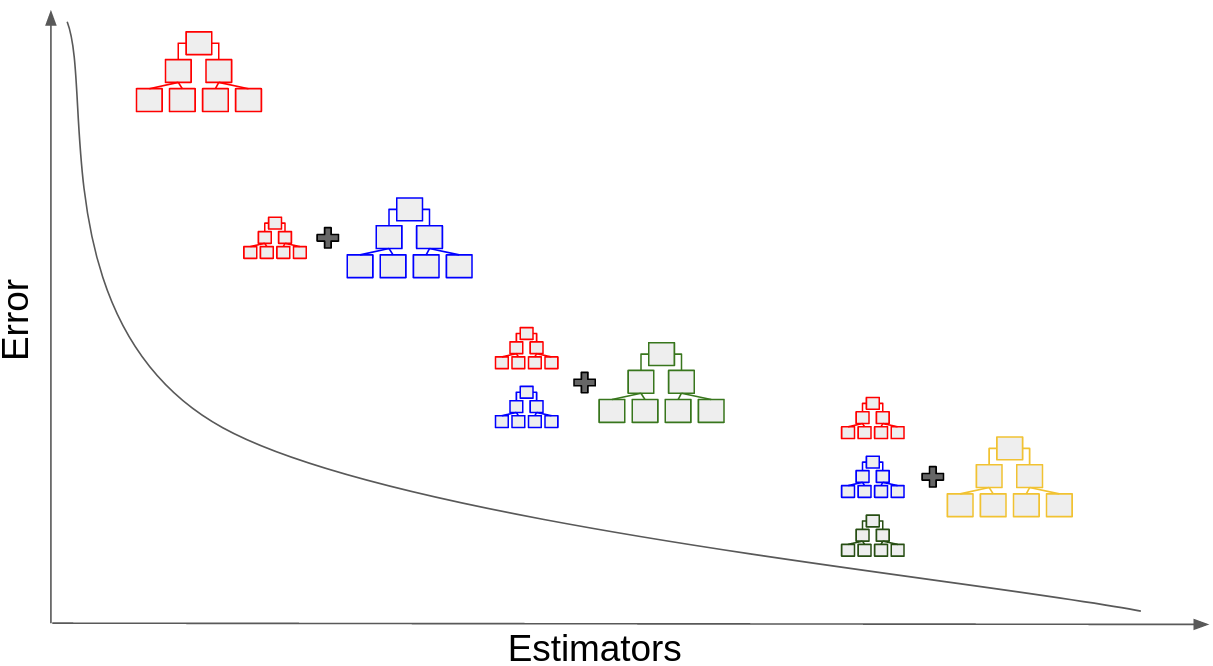
\includegraphics[width=0.75\columnwidth]{Figures/SELD/gbm.png}}
  \caption{Gradient boosting machine learning process. Adding weak estimators allows reducing overall error in the predictions.}
  \label{fig:gbm}
\end{figure}

Sound features are obtained using extractors from \textit{Essentia}, an open-source library for audio analysis \cite{bogdanov2013essentia}. 
Given the heterogeneous nature of the sound classes, a mixture of spectral, temporal and harmonic features are used, as shown in Table~\ref{tab:features}. 
Features are be computed either frame-based or on the whole event; in the former case, the classifier is fed with their temporal first-order statistics. 
% This is the situation for all \textit{Low-level}, and some \textit{SFX} features.
% Conversely, event-level features are passed directly to the classifier. 



\begin{table}[t!]
\caption{Acoustic features used for classification, grouped by type.}
\begin{footnotesize}
\begin{center}
\begin{tabular}{ccc}
\toprule
Type & Features & Number \\
\midrule
\textit{Low-level} & Mel bands & 24       \\
& MFCC & 13 \\
& Spectral Features & 26 \\
% & Pitch Salience &1 \\
\midrule
% SFX & Total and perceived&2 \\
% & sound duration & \\
% & Descriptors based on pitch & 4 \\
% & and harmonics estimation & \\
% & Sound envelope descriptors & 11\\
% & Pitch envelope descriptors & 4\\
\textit{SFX }& Duration &2 \\
& Harmonic & 4 \\
& Sound envelope & 11\\
& Pitch envelope & 4\\
\bottomrule
\end{tabular}
\end{center}
\end{footnotesize}
\label{tab:features}
\end{table}



%%%%%%%%%%%%%%%%%%%%%%%%%%%%%%%%%%%%%%%%%%%%%%%%%%%%%%%%%%%%
%%%%%%%%%%%%%%%%%%%%%%%%%%%%%%%%%%%%%%%%%%%%%%%%%%%%%%%%%%%%

\section{EXPERIMENTS}
\label{sec:experiments}


\subsection{Dataset and baseline system}

The dataset used is the FOA subset of the development set of the \textit{TAU-NIGENS Spatial Sound Events 2020} \cite{politis2020dataset}, which features 600 different B-Format clips of 60 seconds long each. 
Each clip contains multiple sound events, which belong to one of the fourteen sound classes from the NIGENS database \cite{trowitzsch2019nigens}.
Events are also located at a potentially time-varying positions, and the maximum instantaneous overlapping of sources allowed is limited to two. Fifteen different Room Impulse Responses (RIR) are used for scene reverberation, covering a vast range of acoustic conditions. Furthermore, the audio clips contain a moderate amount of recorded background sounds. 

The baseline method is based on the recently proposed SELDnet architecture  \cite{Adavanne2018_JSTSP}, which features a Convolutional Recurrent Neural Network (CRNN) that solves both localization and classification problems jointly. 
Additionally, the baseline implementation has been improved with several changes inspired by one of the best performing methods in DCASE 2019 Task 3 Challenge \cite{Cao2019}. 

\subsection{Experimental setup}


In order to explore the performance of the system, two different approaches have been undertaken regarding the creation of the training dataset for the monophonic single-class classifier. 
The first approach, referred to as \textit{PAPAFIL1}, collects all event localization, temporal activation and class information by parsing the annotation files.
Conversely, the second approach, called \textit{PAPAFIL2}, uses the proposed parametric particle filter to estimate localizations and activations, and the class label is assigned to each event by a custom association algorithm based on spatio-temporal distance. 
In both cases, the input signal is filtered with the obtained information in order to conform the monophonic event estimates.

Therefore, the difference between training datasets is noticeable: while the training events in \textit{PAPAFIL1} are more accurately determined than in \textit{PAPAFIL2}, the differences with respect to the prediction scenario are much bigger in the former case. 
% Consequently, a slightly better performance of the second method might be expected, provided that the parametric particle filter performance has some degree of robustness and accuracy.
The number of individual events for each of the approaches is plotted in Fig.~\ref{fig:num_events}. Approximately half of the classes have similar number of instances in both datasets. However, the other half presents noticeable differences, which might be explained by the different criteria applied for the consideration of event temporal activations: the groundtruth seems to follow a frame-based activity detection approach, while the output of the proposed method tends to consider events as time-continuous manifestations, influenced by the particle filter.

This situation leads to two different \textit{oracle} systems (referred to by appending \textit{-O} in the method name), which represent the best performance theoretically achievable for the corresponding method. 

\begin{figure}[t]
  \centering
  \centerline{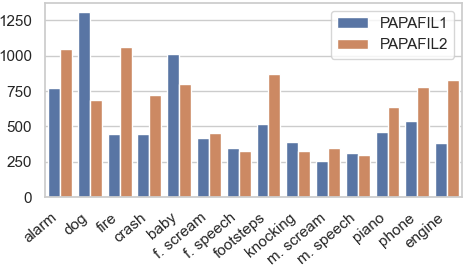
\includegraphics[width=\columnwidth]{Figures/SELD/numclasses2_tight.png}}
  \caption{Number of occurrences of each event class in the training set, for both proposed methods. }
  \label{fig:num_events}
\end{figure}


The accurate information of the \textit{PAPAFIL1} training set suggests a need for data augmentation; 
in contrast, the training material used in \textit{PAPAFIL2} is already provided by a certain extent of variability.
This situation motivates the implementation of data augmentation methods in the \textit{PAPAFIL1} training set.
Specifically, several standard data augmentation techniques are implemented: pitch shifting, time shifting, time stretching and white noise addition.
Furthermore, given the observed high influence of reverberation in the system performance, a reverberant data augmentation technique based on synthetic RIRs has been considered. 
Ten different single-channel RIRs, with reverberation times between 0.3 and 1.1 seconds, have been synthetically created using the \textit{masp} library \cite{perez2020python}. During training, each event estimate is convolved with one of the RIRs, randomly chosen. 
RIR augmentation has recently been shown very effective for blind reverberation time estimation \cite{bryan2020impulse} but, to the best of the authors' knowledge, this is the first application in SELD.

% The presented scheme leads to two different \textit{oracle} systems (named by an \textit{-O} appendix in the method name), which represent the best performance theoretically achievable for the corresponding method. 

% In this way, it is expected that \textit{PAPAFIL1-O} obtains very high localization scores overall, while the performance of \textit{PAPAFIL2-O} can be much similar to the non-oracle case.

% It is important to notice that the spatial filtering is performed with a first-order cardioid, which provides a broad directive pattern. Accordingly, in the case of overlapping events, there will be always signal cross-talk, even when using the groundtruth annotations. The usage of higher ambisonic orders could easily mitigate this effect. 

Table~\ref{tab:parameter} shows a comprehensive list of the parameters used throughout the different steps of the proposed method. All values are equal for both presented approaches, except for the number of Monte-Carlo particles $N$. 
The values for Single-Source Estimation and Particle Filtering parameters have been iteratively refined by manual tuning and inspection, departing from standard values. 
The beamforming weights $\alpha_m$ correspond to the \textit{maximum directivity beamformer}, which minimizes the energy contributions from directions other than the lookup direction \cite{rafaely2015fundamentals}. In the spatial audio field, such property is also known as the \textit{max-rE} decoder \cite{daniel2000representation}. 
Regarding event classification, a cross-validation scheme has been implemented for tuning GBM hyperparameters. 
% In addition, unlike other methods such as CRNN, GBM allows to analyze the relative importance of each feature in the classifier. As it can be seen in Figure \ref{fig:importance}, the most representative variable is sfx.duration, being also important lowlevel.mfcc and spectral variables.

% \begin{figure}[t]
%   \centering
%   \centerline{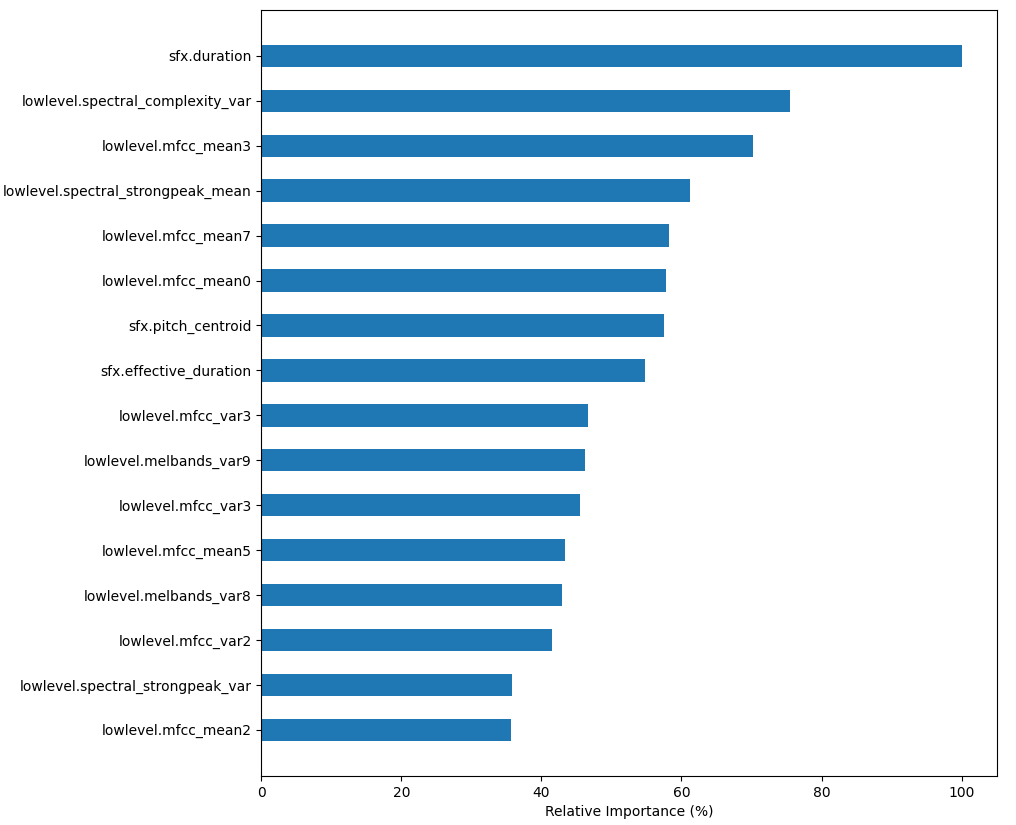
\includegraphics[width=1\columnwidth]{Figure_2.png}}
%   \caption{Most representative features in event classifier }
%   \label{fig:importance}
% \end{figure}



\begin{table}[th!]
\begin{footnotesize}
\caption{(Hyper-)parameter values.}
    \begin{center}
\begin{tabular}{cccc}
\toprule
Step & Parameter & Value & Unit \\
\midrule
Single-Source &sample rate     & 24    &  kHz\\
% Estimation&window type     & hann  &  \\
&window size      & 2400 &  samples\\
&window overlap  & 50  &  \% \\
&$f_{max}$   &  6     &  kHz\\
&$N_\Psi$  & 2     &  frames\\
&$\Psi_{max}$    & 0.1  &  \\

\midrule
Particle & $v$ & 2     &  $^\circ$/frame\\
Filtering & $\sigma_{\nu}$   & 5     &  \\
& $s_{\nu}$ & 20    &  \\
& $p_{birth}$     & 0.25  &  \\
& $p_{\nu}$    & 0.25  &  \\
& $N$  & 100 / 30    &  \\
&$K_{min}$ & 10     &  bins/frame\\ 
&$T_{min}$  & 10     &  frames\\ 

\midrule
Signal & $\alpha_0$     &  0.775 & \\
Filter & $\alpha_1$     &   3 * 0.4 & \\

\midrule
Event & number of estimators   & 1300       & trees  \\
Classification & loss  &  \textit{mlogloss}    &\\
& learning rate & 0.05& \\
& max depth & 4 & \\
& min samples leaf & 10 & samples \\
\bottomrule
\label{tab:parameter}
\end{tabular}
 \end{center}
\end{footnotesize}
\end{table}


%%%%%%%%%%%%%%%%%%%%%%%%%%%%%%
\subsection{Evaluation metrics}

The system is evaluated according to the joint metrics proposed in the Challenge \cite{Mesaros_2019_WASPAA}. 
The metrics evaluate jointly the localization and the classification, and are divided into two types: location-aware classification, and classification-aware localization. 
There are two classification metrics: Error Rate ($\text{ER}_{20}$) and F-Score ($\text{F}_{20}$). As the name suggests, the metrics are conditioned to a minimum localization performance, which is set to 20$^{\circ}$ in this case.
Localization metrics are also two-fold: Localization Error ($\text{LE}_{CD}$) and Localization Recall ($\text{LR}_{CD}$); 
as their name suggests, the metrics are class-dependent, and thus are conditioned to a correct classification.
Finally, the $\text{SELD}$ score is an average of the four other metrics, used to conveniently sum up the results. 




%%%%%%%%%%%%%%%%%%%%%%%%%%%%%%%%%%%%%%%%%%%%%%%%%%%%%%%%%%%%
%%%%%%%%%%%%%%%%%%%%%%%%%%%%%%%%%%%%%%%%%%%%%%%%%%%%%%%%%%%%
\section{RESULTS}
\label{sec:results}

Table~\ref{tab:results} summarizes the results of the experiments using the recommended data split: training with folds 3 to 6, validation with fold 2 and testing with fold 1. 
% This structure has been promoted by the Challenge organization as a fair way for method comparison. 
% Furthermore, the usage of an unseen split 
% Furthermore, it is expected to provide similar results to the evaluation set, given that part of the data remains unseen at training.
Results are reported for three different systems: the baseline and the two proposed methods \textit{PAPAFIL1} and \textit{PAPAFIL2}.
The results of their respective oracle results, \textit{PAPAFIL1-O} and \textit{PAPAFIL2-O}, are also provided. 

Both proposed approaches outperform the baseline system in three out of the four evaluation metrics ($\text{ER}_{20}$, $\text{F}_{20}$ and $\text{LE}_{CD}$). 
Although the results obtained by both of them are similar, \textit{PAPAFIL2} obtains better classification scores ($\text{ER}_{20}$ and $\text{F}_{20}$), and \textit{PAPAFIL1} performs subtly better regarding localization error ($\text{LE}_{CD}$).
However, the localization recall results ($\text{LR}_{CD}$) are slightly worst than the baseline in both cases. This fact does not prevent the proposed methods to have a $\text{SELD}$ score better than the baseline: 0.41 (\textit{PAPAFIL1}) and 0.38 (\textit{PAPAFIL2}), against 0.47 (\textit{BASELINE}).

The results obtained by the oracle methods are within the expected ranges. \textit{PAPAFIL1-O} performs almost perfectly regarding $\text{LE}_{CD}$, but the classification errors influence the $\text{LR}_{CD}$ result.
In turn, \textit{PAPAFIL2-O} performs better than \textit{PAPAFIL1-O} regarding all metrics, excepting $\text{LE}_{CD}$; this improvement is specially noticeable in $\text{LR}_{CD}$, with a performance difference of about 15\%.
The good results obtained by \textit{PAPAFIL2-O} validate the proposed particle filtering approach, an leave space for improvements that might be given by a better understanding and fine tuning of the model.


The performance of the proposed methods deteriorates noticeably with overlapping sounds.
% Although the performance is good in general terms with both \textit{PAPAFIL} approaches, the results deteriorate noticeably with overlapping sounds.
A closer inspection reveals that, in many occasions, the TF bins passing the single-source test mostly belong to one out of two simultaneous sources. 
It is a known issue that performance of DirAC diffuseness is reduced when two sources are present \cite{epain2016spherical}; similar problems have been reported in \cite{adavanne2019localization}, where an instantaneous source number estimator is used in combination with the particle filter.
As in that case, the results suggest the need for more sophisticated source detection and counting methods. 



\begin{table}[th!]
\begin{footnotesize}
\caption{Evaluation results on the development set.}
    \begin{center}
    \begin{tabular}{cccccc}
    \toprule
    Method   & $\text{ER}_{20}$ & $\text{F}_{20}$   & $\text{LE}_{CD}$ & $\text{LR}_{CD}$ & $\text{SELD}$ \\
    \midrule
    \textit{BASELINE} & 0.72   & 37.4 \% & 22.8$^{\circ}$ & \textbf{60.7} \% & 0.47 \\
    \textit{PAPAFIL1} & 0.60 & 49.8 \% & \textbf{13.4}$^{\circ}$ & 54.4 \% &0.41\\

    \textit{PAPAFIL2} & \textbf{0.57} & \textbf{54.0} \% &13.8$^{\circ}$ & 59.7 \% & \textbf{ 0.38} \\
    
    \midrule
    % this is oracle beam
    \textit{PAPAFIL1-O} & 0.37 & 67.0 \% & 2.0$^{\circ}$ & 68.6 \% & 0.26 \\
    \textit{PAPAFIL2-O} & 0.32 & 79.6 \% & 8.5$^{\circ}$ & 82.4\% & 0.19 \\
    
    % \midrule
    % \textit{PAPAFIL1} &  0.57 & 55.6 \% & 15.6$^{\circ}$ & 66.7 \% & 0.36 \\
    % % PAPAFIL_1 & 0.47  & 64.1 \% & 14.1$^{\circ}$ & 70.1 \% & 0.30 \\ ?????????
    % % this is oracle beam
    % \textit{PAPAFIL1-O} & 0.08 & 93.7 \% &  0.2$^{\circ}$ & 94.0 \% & 0.05 \\
    
    %  \textit{PAPAFIL2} & \textbf{ 0.44} & \textbf{68.0} \% & \textbf{13.3}$^{\circ}$ & \textbf{79.6} \% & \textbf{0.26} \\
    
    % \textit{PAPAFIL2-O} & 0.41 & 71.1 \% & 12.3$^{\circ}$ & 82.0\% &  0.24 \\
    \bottomrule
    \end{tabular}
    \end{center}
    \label{tab:results}
\end{footnotesize}
\end{table}

\begin{figure}[t]
  \centering
  \centerline{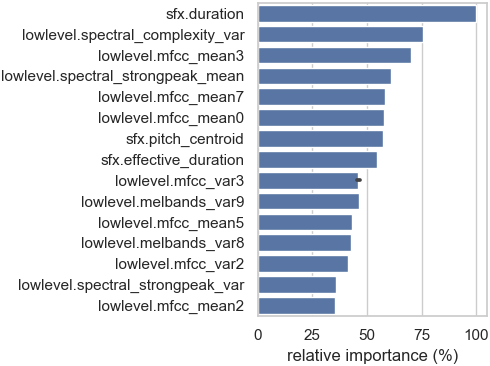
\includegraphics[width=\columnwidth]{Figures/SELD/importance_new_tight.png}}
  \caption{Most representative features in event classifier.}
  \label{fig:importance}
\end{figure}

To conclude the analysis, Fig.~\ref{fig:importance} shows the relative importance of the fifteen most relevant acoustic features for the \textit{PAPAFIL2} classifier model.
Event duration is clearly the feature with the highest importance, and effective duration (duration of the signal discarding silence) also appears in the eighth position.
This fact can help to explain the better performance of \textit{PAPAFIL2} over \textit{PAPAFIL1}: the temporal activities of the events in training and prediction are much more similar to each other in the former method, as a consequence of the training set generation approach.
Furthermore, it is interesting to notice the high relevance of low-level features, and specifically several MFCC combinations (eight of the fifteen reported features) and  various extractors related to the spectral structure. The absence of pitch, harmonic and envelope features in the list represents a significant finding as well. 



\todo{TODO: DISCUSS RESULTS OF EVALUATION SET!!}




%%%%%%%%%%%%%%%%%%%%%%%%%%%%%%%%%%%%%%%%%%%%%%%%%%%%%%%%%%%%
%%%%%%%%%%%%%%%%%%%%%%%%%%%%%%%%%%%%%%%%%%%%%%%%%%%%%%%%%%%%
\section{Conclusion}
\label{sec:results}

% We have presented a novel method for Sound Event Localization and Detection (SELD), based on parametric particle filtering and gradient boosting single-class event classification of audio features. Results show that the proposed method outperforms the baseline method, a state-of-the-art Convolutional Recurrent Neural Network (CRNN). Specifically, the proposed method is able to improve the baseline SELD score by almost ten points, while also increasing the evaluation score in three out of the four proposed metrics, by means of a low complexity machine learning architecture.

We present a novel low-complexity method for Sound Event Localization and Detection of First Order Ambisonic signals, based on four steps: estimation of single-source spectrogram regions by parametric analysis; computation of event trajectories and activations by means of a particle tracker; spatio-temporal filtering of the input signal; and single-class monophonic event classification by Gradient Boosting. 
Results show that the proposed method outperforms the baseline method, a state-of-the-art Convolutional Recurrent Neural Network. Specifically, our method is able to improve the baseline SELD score by almost ten points, while increasing the scores in three out of the four metrics under consideration.

%%%%%%%%%%%%%%%%%%%%%%%%%%%%%%%%%%%%%%%%%%%%%%%%%%%%%%%%%%%%
%%%%%%%%%%%%%%%%%%%%%%%%%%%%%%%%%%%%%%%%%%%%%%%%%%%%%%%%%%%%
%%%%%%%%%%%%%%%%%%%%%%%%%%%%%%%%%%%%%%%%%%%%%%%%%%%%%%%%%%%%
%%%%%%%%%%%%%%%%%%%%%%%%%%%%%%%%%%%%%%%%%%%%%%%%%%%%%%%%%%%%
%%%%%%%%%%%%%%%%%%%%%%%%%%%%%%%%%%%%%%%%%%%%%%%%%%%%%%%%%%%%
%%%%%%%%%%%%%%%%%%%%%%%%%%%%%%%%%%%%%%%%%%%%%%%%%%%%%%%%%%%%
%%%%%%%%%%%%%%%%%%%%%%%%%%%%%%%%%%%%%%%%%%%%%%%%%%%%%%%%%%%%
%%%%%%%%%%%%%%%%%%%%%%%%%%%%%%%%%%%%%%%%%%%%%%%%%%%%%%%%%%%%
%%%%%%%%%%%%%%%%%%%%%%%%%%%%%%%%%%%%%%%%%%%%%%%%%%%%%%%%%%%%
%%%%%%%%%%%%%%%%%%%%%%%%%%%%%%%%%%%%%%%%%%%%%%%%%%%%%%%%%%%%
%%%%%%%%%%%%%%%%%%%%%%%%%%%%%%%%%%%%%%%%%%%%%%%%%%%%%%%%%%%%
%%%%%%%%%%%%%%%%%%%%%%%%%%%%%%%%%%%%%%%%%%%%%%%%%%%%%%%%%%%%
%%%%%%%%%%%%%%%%%%%%%%%%%%%%%%%%%%%%%%%%%%%%%%%%%%%%%%%%%%%%
%%%%%%%%%%%%%%%%%%%%%%%%%%%%%%%%%%%%%%%%%%%%%%%%%%%%%%%%%%%%
%%%%%%%%%%%%%%%%%%%%%%%%%%%%%%%%%%%%%%%%%%%%%%%%%%%%%%%%%%%%
%%%%%%%%%%%%%%%%%%%%%%%%%%%%%%%%%%%%%%%%%%%%%%%%%%%%%%%%%%%%

%\section{Introduction}
%\label{sec:intro}
%
%Sound Event Localization and Detection (SELD) refers to the problem of identifying, for each individual  event present in a sound field, the temporal activity, spatial location, and sound class to which it belongs. SELD is a current research topic which deals with microphone array processing and sound classification, with potential applications in the fields of signal enhancement, autonomous navigation, acoustic scene description or surveillance, among others.
%
%SELD arises from the combination of two different problems: Sound Event Detection (SED) and Direction of Arrival (DOA) estimation. The number of works in the literature which jointly address SED and DOA problems is relatively small. It is possible to classify them by the type of microphone arrays used: distributed \cite{grobler2017sound, butko2011two, chakraborty2014sound} or near-coincident \cite{hirvonen2015classification, lopatka2016detection, Adavanne2018_JSTSP}.
%As mentioned in \cite{Adavanne2018_JSTSP}, the usage of near-coincident circular/spherical arrays enables the representation of the sound field in the spatial domain, using the spherical harmonic decomposition, also known as Ambisonics \cite{gerzon1973periphony, daniel2000representation}. Such spatial representation allows a flexible, device-independent comparison between methods. Furthermore, the number of commercially available ambisonic microphones has increased in recent years due to their suitability for immersive multimedia applications.  
%Taking advantage of the compact spatial representation provided by the spherical harmonic decomposition, several methods for parametric analysis of the sound field in the ambisonic domain have been proposed  \cite{pulkki2006directional, berge2010high, Politis2018, pulkki2018parametric}.
%These methods ease sound field segmentation into direct and diffuse components, and further localization of the direct sounds.
%The advent of deep learning techniques for DOA estimation has also improved the results of traditional methods \cite{Adavanne2018_JSTSP}. However, none of the deep learning-based DOA estimation methods explicitly exploits the spatial parametric analysis. This situation is further extended to the SELD problem, with the exception of \cite{lopatka2016detection}, where DOAs are estimated from the \textit{active intensity vector}  \cite{pulkki2006directional}.
%
%The motivation for the proposed methodology is two-fold.
%First, we would like to check whether the usage of spatial parametric analysis in the ambisonic domain can improve the performance of SELD algorithms.
%Second, temporal information derived by the parametric analysis could be further exploited to estimate event onsets and offsets, thus lightening the event classifier complexity; such reduction might positively impact algorithm's performance.
%
%In what follows, we present the methodology and the architecture of the proposed system (Section~\ref{sec:method}). Then, we describe the design choices and the experimental setup (Section~\ref{sec:expe}), and discuss the results in the context of DCASE2019 Challenge - Task 3 (Section~\ref{sec:results}). A summary is presented in Section~\ref{sec:conclusion}. 
%%In order to support open access and reproducibility, all code is freely available at \cite{code}. \todo{code ref}.
%
%
%\section{Method}
%\label{sec:method}
%
%The proposed method presents a solution for the SELD problem splitting the task into four different problems: \textit{DOA  estimation}, \textit{association}, \textit{beamforming} and \textit{classification}, which will be described in the following subsections.
%The former three systems follow a heuristic approach---in what follows, they will be jointly referred to as the \textit{parametric front-end}. Conversely, the \textit{classification} system is data-driven, and will be referred to as the \textit{deep learning back-end}. The method architecture is depicted in Figure~\ref{fig:diagram_all}.
%
%\todo{redo figures in this section}
%
%\begin{figure}[h]
%	\centering
%    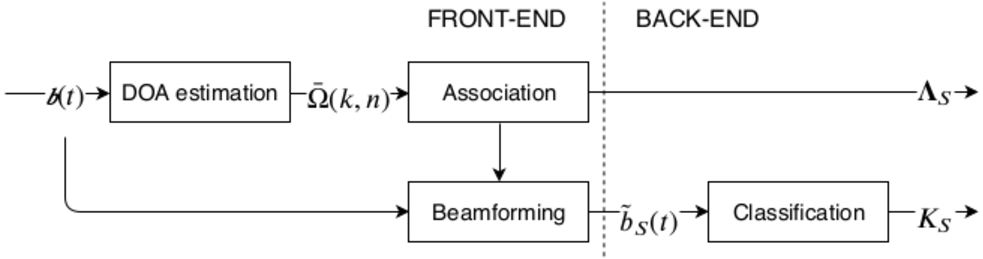
\includegraphics[width=\columnwidth]{Figures//SELD/dcase_challenge_tech_report_all2.pdf}
%    \caption{System architecture.}
%    \label{fig:diagram_all}
%
%\end{figure}
%
%\subsection{DOA estimation}
%\label{ssec:doa_estimation}
%
%\begin{figure*}[h]
%
%    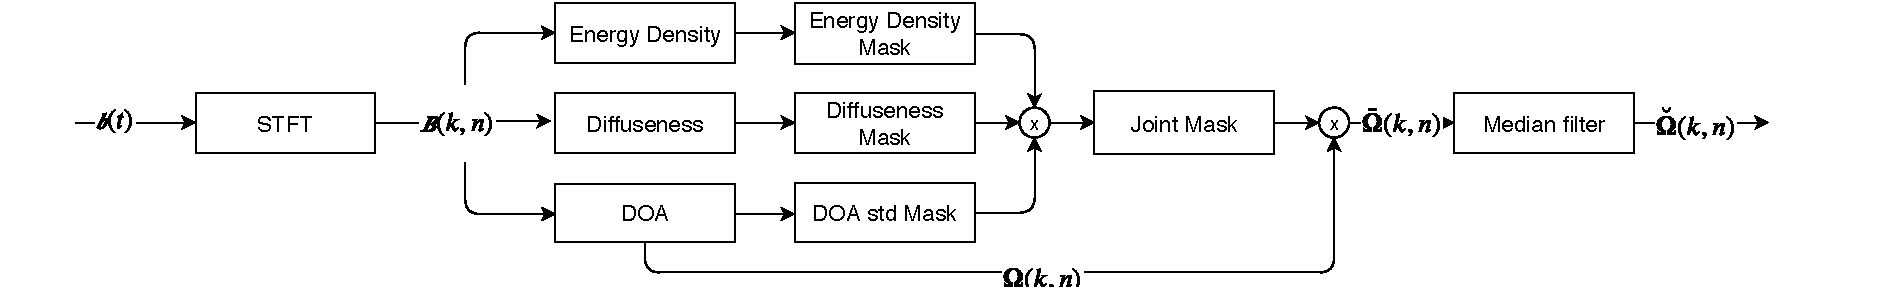
\includegraphics[width=\textwidth]{Figures/SELD/DOA1.pdf}
%    \caption{DOA estimation architecture.}
%    \label{fig:doa}
%
%\end{figure*}
%
%
%
%The \textit{DOA estimation} system (Figure~\ref{fig:doa}) is based on parametric time-frequency spatial audio analysis.
%
%Let us consider a \textit{N3D}-normalized first-order ambisonic signal $x_n^m(t)$. 
%Using the DirAC parametric model, it is possible to obtain instantaneous time-frequency estimates of the Direction of Arrival $\Omega(k,n)$ (Eq.~\ref{eq:doa}), energy density $E(k,n)$ (Eq.~\ref{eq:energydensity}) and the diffuseness $\Psi(k,n)$ (Eq.~\ref{eq:psidefinition}).\\
%
%
%
%%Let us consider a first order ambisonic signal $$
%%Let us consider a first order ambisonic signal vector $\pmb{b}(t)$ with N3D normalization \cite{carpentier2017normalization}:
%%\begin{equation}
%%    \pmb{b}(t) = [b_w(t), \sqrt{3}b_x(t),\sqrt{3}b_y(t), \sqrt{3}b_z(t)].
%%\end{equation}
%%From its short-time frequency domain representation $\pmb{B}(k,n)$, the instantaneous DOA at each TF bin $\pmb{\Omega}(k,n)$ can be estimated as:
%%\begin{equation}
%%    \begin{aligned}
%%    \pmb{I}(k,n) = -\frac{1}{Z_0}\mathbb{R}\{& [B_x(k,n), B_y(k,n), B_z(k,n)]  B_w(k,n)^* \},\\
%%    \pmb{\Omega}(k,n) &= [\varphi(k,n), \theta (k,n)] =\angle ( -\pmb{I}(k,n) ),
%%    \end{aligned}
%%\end{equation}
%%where $\pmb{I}(k,n)$ stands for the \textit{active intensity vector} \cite{pulkki2006directional}, $Z_0$ is the characteristic impedance of the medium, $^*$ represents the complex conjugate operator, and $\angle$ is the spherical coordinates angle operator, expressed in terms of azimuth $\varphi$ and elevation $\theta$.
%
%It is desirable to identify the TF regions of $\Omega(k,n)$ which carry information from the sound events, and discard the rest. Three binary masks are computed with that aim.
%
%The first mask is the \textit{energy density mask}, which is used as an activity detector. A gaussian adaptive thresholding algorithm is applied to $E(k,n)$. This procedure selects TF bins with local maximum energy density, as expected from the direct path of the sources.
%
%The \textit{diffuseness mask} selects the TF bins with high energy propagation. Bins with a low diffuseness value represent a TF region where one sound source is predominant. A fixed threshold value $\Psi_{max}$ is used for the masking.
%
%The third mask is the \textit{DOA variance mask}. It tries to select TF regions with small standard deviation with respect to their neighbor bins---a characteristic of sound fields with low diffuseness \cite{pulkki2018parametric}.\\
%
%The three masks are then applied to the DOA estimation, obtaining the TF-filtered instanteneous DOAs $\bar{\Omega}(k,n)$. 
%Finally, a median filter is applied, with the aim of improving DOA estimation consistency and removing spurious TF bins.
%The median filter is applied in a TF bin belonging to $\bar{\Omega}(k,n)$ only if the number of TF bins belonging to $\bar{\\Omega}(k,n)$ in its vicinity is greater than a given threshold $B_{min}$.
%The resulting filtered DOA estimation is referred to as $\breve{\Omega}(k,n)$.
%
%
%\subsection{Association}
%\label{ssec:association}
%
%\begin{figure*}[h]
%    
\includegraphics[width=\textwidth]{Figures/SELD//ASS.pdf}
%    \caption{Association architecture.}
%    \label{fig:association}
%
%\end{figure*}
%
%The association step (Figure~\ref{fig:association}) tackles the problem of assigning the time-frequency-space observation $\breve{\Omega}(k,n)$ to a set of events, each one having a specific onset, offset and location. \\
%
%First, DOA estimates are resampled into \textit{frames} with the task's required length ($0.02$ s). In what follows, frames will be represented by index $m$. 
%An additional constraint is applied: for a given window $n_0$, the DOA estimates $\breve{\Omega}(k,n_0)$ are assigned to the corresponding frame $m_0$ only if the number of estimates is higher than a given threshold $K_{min}$.\\
%
%Next, the standard deviation in azimuth $\sigma_{\varphi}$ and elevation $\sigma_{\theta}$ of the frame-based DOA estimates $\breve{\Omega}(k,m)$ are compared to a threshold value $\sigma_{max}$, and the result is used to estimate the frame-based event overlapping amount $o(m)$ :
%
%\begin{equation}
%\begin{aligned}
%	o(m) =  \begin{cases}
%    		1, &\text{if } \sigma_{\varphi}/2 + \sigma_{\theta} < \sigma_{max},\\
%    		2, &\text{otherwise}.
%    \end{cases}    		
%\end{aligned}
%\end{equation}
%
%The clustered values $\Omega_{\text{cluster}}(m)$ are then computed as the $K=o(m)$ centroids of $\breve{\Omega}(k,m)$, using a modified version of K-Means which minimizes the central angle distance. Notice that, for $o(m)=1$, the operation is equivalent to the median.\\
%
%The following step is the grouping of clustered DOA values into events.
%Let us define $\Omega_S(m)$ as the frame-wise DOA estimations belonging to the event $S$. A given clustered DOA estimation $\Omega_{\text{cluster}}(m)$ belongs to the event $S$ if the following criteria are met:
%\begin{itemize}
%    \item The central angle between  $\Omega_{\text{cluster}}(m)$ and the median of $\Omega_S(m)$ is smaller than a given threshold $d_{max}^\text{ANGLE}$, and
%    \item The frame distance between $m$ and the closest frame of $\Omega_S(m)$ is smaller than a given threshold $d_{max}^\text{FRAME}$.
%\end{itemize}
%
%The resulting DOAs $\Omega_S(m)$ are subject to a postprocessing step with the purpose of 
%delaying event onsets in frames where $o(m) > 2$, and discarding events shorter than a given minimum length. 
%
%Finally, the frame-based event estimations are converted into \textit{metadata annotations} in the form $\Lambda_S = (\Omega_S, \text{onset}_S, \text{offset}_S)$.
%
%\subsection{Beamforming}
%\label{ssec:Beamforming}
%
%The last step performed in the front-end is the input signal segmentation. The spatial and temporal information provided by the annotations $\Lambda_S$ are used to produce monophonic signal estimations of the events, $\tilde{x}_S(t)$, as the signals captured by a virtual first-order cardioid (Eq.~\ref{eq:decodingequation}):
%\begin{equation}
%\tilde{x}_S(t) = x_n^m(t) Y_n^m(\Omega_S) \alpha_n,
%\end{equation}
%with $\alpha_n = [1, 1, 1, 1]$ using the \textit{basic} decoding weights.
%
%
%
%\subsection{Deep learning classification back-end}
%\label{ssec:backend_method}
%
%%intro - problem formulation==============
%The parametric front-end performs DOA estimation, temporal activity detection and time/space segmentation, and produces monophonic estimations of the events, $\tilde{s}_S(t)$.
%Then, the back-end classifies the resulting signals as belonging to one of a target set of 11 classes.
%Therefore, the multi-task nature of the front-end allows us to define the back-end classification task as a simple multi-class problem, even though the original SELD task is multi-label.
%It must be noted, however, that due to the limited directivity of the first-order beamformer, the resulting monophonic signals can present a certain leakage from additional sound sources when two events overlap, even when the annotations $\Lambda_S$ are perfectly estimated.
%
%%2 stages: context
%The classification method is divided into two stages.
%First, the incoming signal is transformed into the log-mel spectrogram and split into TF patches.
%Then, the TF patches are fed into a single-mode based on a Convolutional Recurrent Neural Network (CRNN), which outputs probabilities for event classes $c \in \left\lbrace 1 ...C \right\rbrace$, with $C=11$.
%Predictions are done at the event-level (not at the frame level), since the temporal activities have been already determined by the front-end.
%Only one label is predicted for each incoming event, such that there is no binarization stage needed as in a standard SED task.
%
%%archi=============
%The proposed CRNN is depicted in Figure \ref{fig:archi}.
%It presents three convolutional \textit{blocks} to extract local features from the input representation.
%Each convolutional block consists of one convolutional layer, after which the resulting feature maps are passed through a ReLU non-linearity \cite{nair2010rectified}.
%This is followed by a max-pooling operation to downsample the feature maps and add invariance along the frequency dimension.
%The target classes vary to a large extent in terms of their temporal dynamics, with some of them being rather impulsive (e.g., \textit{Door slam}), while others being more stationary (e.g., \textit{Phone ringing}). 
%Therefore, after stacking the feature maps resulting from the convolutional blocks, this representation is fed into one bidirectional recurrent layer in order to model discriminative temporal structures.
%Specifically, 64 nodes of gated recurrent units (GRU) are used with \textit{tanh} activations.
%The recurrent layer is followed by a Fully Connected (FC) layer, and finally a 11-way softmax classifier layer produces the event-level probabilities.
%Dropout is applied extensively.
%The loss function used is categorical cross-entropy.
%The model has $\sim$175k weights.
%
%\begin{figure}[ht]
%  \vspace{-3mm}
%  \centering
%  \centerline{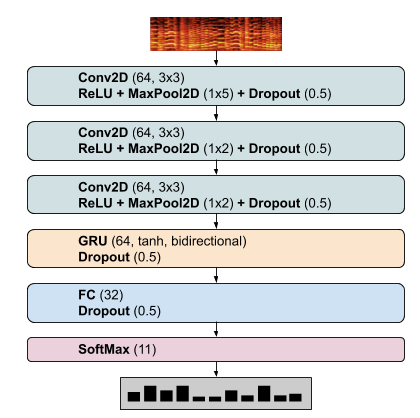
\includegraphics[width=0.9\textwidth]{Figures/SELD/DCASE19Task3_backend_archi_v3.png}}
%  \vspace{-2mm}
%  \caption{Back-end architecture.}
%  \label{fig:archi}
%    \vspace{-5mm}
%\end{figure}
%
%
%
%
%%===============================================================================
%
%\section{Experiments}
%\label{sec:expe}
%
%\subsection{Dataset, evaluation metrics and baseline system}
%\label{ssec:dataset}
%We use the TAU Spatial Sound Events 2019 - Ambisonic, which provides first-order ambisonic recordings.
%Details about the recording format and dataset specifications can be found in \cite{Adavanne2019_DCASE}.
%The dataset features a vocabulary of $C=11$ classes encompassing human sounds and sound events typically found in indoor office environments.
%The dataset is split into a development and evaluation sets. 
%The development set consists of a four fold cross-validation setup.\\
%
%The SELD task is evaluated with individual metrics for the SED and DOA problems:
%\begin{itemize}
%	\item SED: F-score (\textit{F}) and error rate (\textit{ER}) calculated in one-second segments.
%	\item DOA: DOA error (\textit{DOA}) and frame recall (\textit{FR}) calculated frame-wise.
%\end{itemize}
%The \textit{SELD score} is an averaged summary of the system performance.
%A more detailed description of the evaluation metrics can be found in \cite{Adavanne2018_JSTSP}.\\
%
%The baseline system features a CRNN that jointly performs DOA and SED through multi-task learning \cite{Adavanne2018_JSTSP}.
%Baseline results are shown in Table \ref{tab:results_real}.
%
%
%\subsection{Parametric front-end}
%\label{ssec:param_frontend}
%
%Based on the method's exploratory analysis, we propose the following set of parameter values, which are shown in Table~\ref{tab:params_front}.
%
%
%\begin{table}[!htbp]
%
%\centering
%\caption{Parameter values for the selected configuration. Top: \textit{DOA analysis} parameters. Bottom: \textit{Association} parameters.}
%\begin{tabular}{cccc}
%\toprule
%Parameter & Unit & Value\\
%\midrule
%sampling rate & Hz  & 48000\\
%STFT window size & sample  & 256\\
%STFT window overlap & sample & 128\\
%STFT window type & -  &  Hann\\
%analysis frequency range & Hz & [0,8000]\\
%time average vicinity radius $r$ & bin& 10 \\
%diffuseness mask threshold $\Psi_{max}$ & - & 0.5 \\
%energy density filter length & bin & 11\\
%std mask vicinity radius & bin &  2\\
%std mask normalized threshold & - & 0.15\\
%median filter minimum ratio $B_{min}$ & - & 0.5 \\
%median filter vicinity radius (k,n) & bin & (20, 20) \\
%\midrule
%frame size $h$ & s  & 0.02\\
%resampling minimum valid bins $K_{min}$ & bin & 1 \\
%overlapping std threshold $\sigma_{max}$ & degree & 10 \\
%grouping maximum angle $d_{max}^\text{ANGLE}$ & degree & 20\\
%grouping maximum distance $d_{max}^\text{FRAME}$ & frame & 20\\
%event minimum length & frame & 8\\
%\bottomrule
%\end{tabular}
%\label{tab:params_front}
%\end{table}
%
%
%\subsection{Deep learning classification back-end}
%\label{ssec:backend_experiments}
%
%We use the provided four fold cross-validation setup.
%Training and validation stages use the outcome of an \textit{ideal} front-end, where the groundtruth DOA estimation and activation times are used to feed the beamformer for time-space segmentation.
%Conversely, we test the trained models with the signals coming from the \textit{complete} front-end described in Section \ref{sec:method}.
%
%We conducted a set of preliminary experiments with different types of networks including a VGG-like net, a less deep CNN \cite{Fonseca2019learning}, a Mobilenetv1 \cite{howard2017mobilenets} and a CRNN \cite{cakir2017convolutional}.
%The latter was found to stand out, and we explore certain facets of the CRNN architecture and the learning pipeline.\\
%
%Sound events in the dataset last from $\sim$ 0.2 to 3.3 s.
%First, clips shorter than 2s are replicated to meet this length.
%Then, we compute TF patches of log-mel spectrograms of $T=50$ frames (1 s) and $F=64$ bands.
%The values come from the exploration of $T \in \left\lbrace 25,50,75,100\right\rbrace$ and $F \in \left\lbrace 40,64,96,128\right\rbrace$.
%$T=50$ is the top performing value, roughly coinciding with the median event duration. In turn, more than 64 bands provide inconsistent improvements, at the cost of increasing the number of network weights.\\
%
%Regarding the network structure, several variants of the CRNN architecture were explored until reaching the network of Figure \ref{fig:archi}.
%This included a small grid search over number of CNN filters, CNN filter size and shape, number of GRU units, number of FC units, dropout \cite{srivastava2014dropout}, learning rate, and the usage of Batch Normalization (BN) \cite{ioffe2015batch}.
%Network extensions (involving more weights) were considered only if providing major improvements, as a measure against overfitting.
%The main takeaways are: \textit{i)} squared 3x3 filters provide better results than larger filters, \textit{ii)} dropout of 0.5 is critical for overfitting mitigation, \textit{iii)} more than one recurrent layer does not yield improvements, while slowing down training, and \textit{iv)} surprisingly, slightly better performance is attained without BN nor pre-activation \cite{fonseca2018simple}. \\
%
%For all experiments, the batch size was 100 and Adam optimizer was used \cite{kingma2014adam} with initial learning rate of 0.001, halved each time the validation accuracy plateaus for 5 epochs.
%Earlystopping was adopted with a patience of 15 epochs, monitoring validation accuracy.
%Prediction for every event was obtained by computing predictions at the patch level, and aggregating them with the geometric mean to produce a clip-level prediction. \\
%
%
%Finally, we apply \textit{mixup} \cite{zhang2017mixup} as data augmentation technique.
%Mixup consists in creating virtual training examples through linear interpolations in the feature space, assuming that they correspond to linear interpolations in the label space.
%Essentially, virtual TF patches are created on the fly as convex combinations of the input training patches, with a hyper-parameter $\alpha$ controlling the interpolation strength.
%Mixup has been proven successful for sound event classification, even in adverse conditions of corrupted labels \cite{Fonseca2019model}.
%It seems appropriate for this task since the front-end outcome can present leakage due to overlapping sources, effectively mixing two sources while only one training label is available, which can be understood as a form of label noise \cite{Fonseca2019learning}.
%Experiments revealed that mixup with $\alpha=0.1$ boosted testing accuracy in $\sim1.5$\%. 
%
%
%
%
%
%
%%==============================================
%
%\section{Results and Discussion}
%\label{sec:results}
%\begin{table}[!htbp]
%\centering
%\caption{Results for development (top) and evaluation (bottom) sets.}
%
%\begin{tabular}{cccccc}
%\toprule
%Method & \textit{ER} & \textit{F} & \textit{DOA} & \textit{FR} & \textbf{\textit{SELD}}\\
%\midrule
%Baseline & 0.34 & 79.9\% & 28.5$^{\circ}$  & 85.4\% & 0.2113\\
%Proposed & 0.32 & 79.7\% & 9.1$^{\circ}$   & 76.4\% & \textbf{0.2026}\\
%Ideal front-end & 0.08 & 93.2\% & $\sim0^{\circ}$   &$ \sim100$\% & 0.0379\\
%\midrule
%Baseline & 0.28 & 85.4\% & 24.6$^{\circ}$  & 85.7\% &  0.1764\\
%Proposed & 0.29 & 82.1\% & 9.3$^{\circ}$   & 75.8\% & \textbf{ 0.1907}\\
%\bottomrule
%\end{tabular}
%\label{tab:results_real}
%\end{table}
%
%
%Table~\ref{tab:results_real} shows the results of the proposed method for both development and evaluation sets, compared to the baseline.
%Focusing on evaluation results, our method and the baseline obtain similar performance in SED (\textit{ER} and \textit{F}). However, there is a clear difference in the DOA metrics:
%in our method, \textit{DOA} error is reduced by a factor of 2.6, but \textit{FR}  is $\sim10$ points worst.
%In terms of \textit{SELD score}, our method performs slightly worse than the baseline in evaluation mode, while marginally outperforming it in development mode. \\m,              
%
%The most relevant observation is the great improvement in \textit{DOA} error. Results suggest that using spatial audio parametric analysis as a preprocessing step can help to substantially improve localization. 
%Figure \ref{fig:5a} provides further evidence for this argument: Challenge methods using some kind of parametric preprocessing (\textit{GCC-PHAT} with the microphone dataset, and \textit{Intensity Vector-Based} in ambisonics) obtained in average better \textit{DOA} error results. \\
%
%\begin{figure}
%  \begin{subfigure}[b]{\textwidth}
%    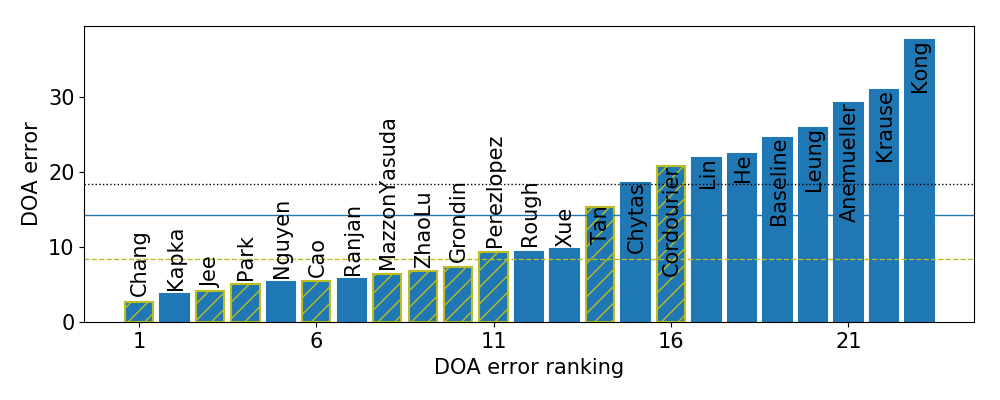
\includegraphics[width=\textwidth]{Figures/SELD//doaerror2.jpg}
%    \caption{\textit{DOA error} across submissions. Hatched bars denote methods using parametric preprocessing. Horizontal lines depict average DOA error accross different subsets: all methods (solid), parametric methods (dashed), non-parametric methods (dotted).}
%    \label{fig:5a}
%  \end{subfigure}
%  \begin{subfigure}[b]{\textwidth}
%    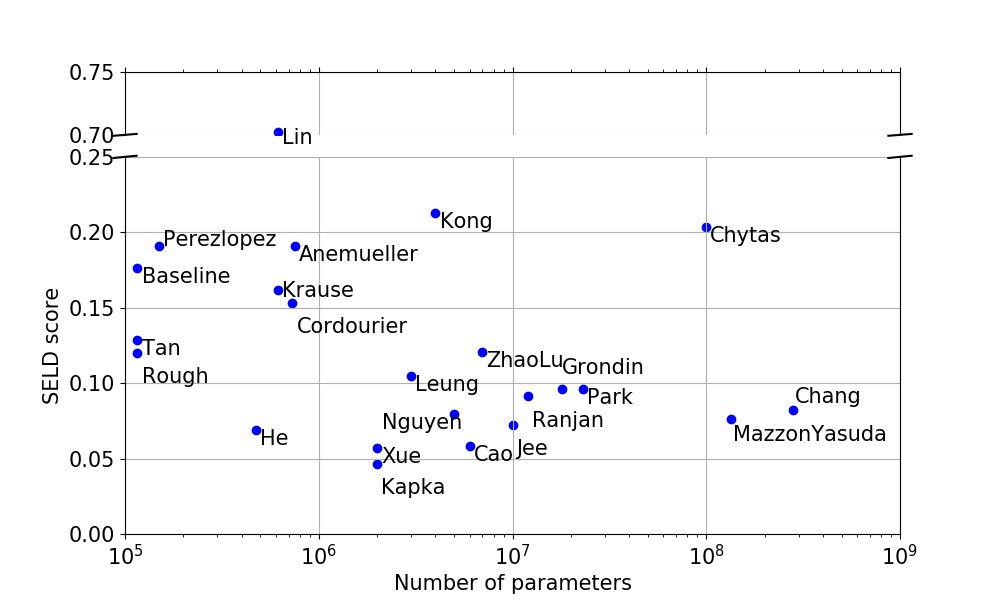
\includegraphics[width=\textwidth]{Figures/SELD//complexity_vs_seld2.jpg}
%    \caption{\textit{SELD score} versus complexity.}
%    \label{fig:5b}
%  \end{subfigure}
%\caption{DCASE2019 Challenge Task 3 results, evaluation set.}
%\end{figure}
%
%Conversely, the front-end fails regarding \textit{FR}. This is probably due to the complexity added by the association step \cite{Adavanne2018_JSTSP}, and its lack of robustness under highly reverberant scenarios. Including spectral information at the grouping stage might help to improve \textit{FR} --- such information could be provided by the classification back-end, in a similar approach to the baseline system. Another option would be the usage of more sophisticated source counting methods \cite{he2010detecting, Stefanakis2017}. \\
%
%In order to gain a better insight of the classification back-end performance, Table~\ref{tab:results_real} shows the method results when the testing clips are obtained by feeding  the beamformer  with groundtruth annotations (\textit{ideal} front-end).
%In this ideal scenario of DOA performance, the SED metrics show a significant boost. 
%This result suggests that the low \textit{FR} given by the front-end has a severe impact on the back-end  performance.
%Yet, the proposed system reaches similar performance to the baseline system in terms of SED metrics. \\
%
%Finally, we would like to discuss algorithm complexity among Challenge methods. 
%As depicted in Figure \ref{fig:5b}, there is a general trend towards architectures with very high number of weights, as a consequence of the usage of ensembles and large capacity networks.
%Specifically, 66\% of submitted methods employ 1M weights or more, 30\% employ 10M or more, and 15\% employ 100M or more. Such complexities are several orders of magnitude greater than the baseline (150k weights) or the proposed method ($\sim$175k weights).
%In this context, our method represents a low-complexity solution to the SELD problem, featuring a number of parameters and a performance comparable to the baseline method.
%
%
%\section{Conclusion}
%\label{sec:conclusion}
%
%We present a novel approach for the SELD task. Our method relies on spatial parametric analysis for the computation of event DOAs, onsets and offsets. This information is used to filter the input signals in time and space, and the resulting event estimations are fed into a CRNN which predicts the class to which the events belong; the classification problem is thereby handled from a simple multi-class perspective.
%The proposed method is able to obtain an overall performance comparable to the baseline system. 
%The localization accuracy achieved by our method greatly improves the baseline performance, suggesting that spatial parametric analysis might enhance performance of SELD algorithms. Moreover, detection and classification performance in our method suffers from a low Frame Recall; improving this metric could lead to promising SELD scores.
%
%
%
